\subsection{Eigenspace Overlap of Different Models}
\label{sec:appendix_model_overlap}
% \begin{figure}[ht]
%     \centering
%     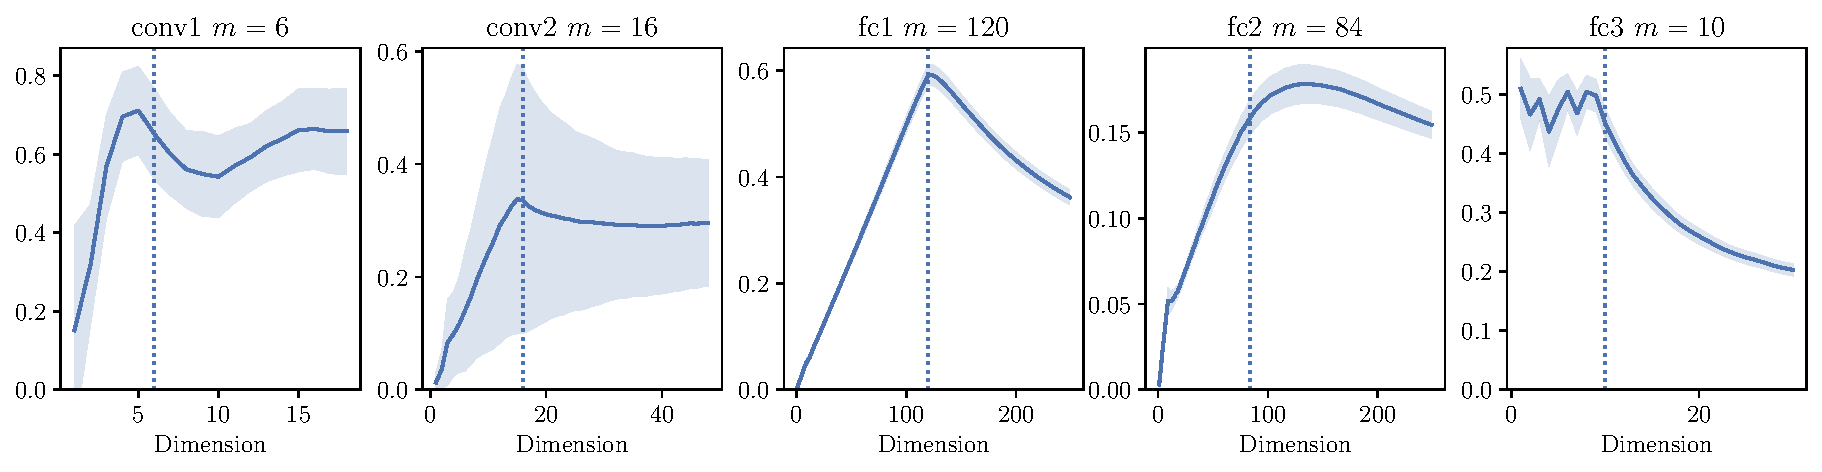
\includegraphics[width=\textwidth]{Appendix_Figures/Overlap_different_models/DimOverlap_CIFAR10_LeNet5_normnew_fixlr0.01_appendix_full.pdf}
%     \caption{Eigenspace overlap of different models of LeNet5}
%     \label{fig:app_adexp_lenet5_fixlr0.01}
% \end{figure}
% %In this section we explain
% %\begin{enumerate}
%     %\item linear growth (in general) and why no linear growth for fc3
%     %\item why fc2 bad (M too low rank)
%     %\item why conv1 high
%     %\item why fc2 still exhibits a linear segment at the begining.
% %\end{enumerate}
% \figureref{fig:app_adexp_lenet5_fixlr0.01} shows the average pairwise overlap between the top eigenspaces of the layer-wise Hessian of 5 different LeNet5 models.
From the experiment results in \sectionref{sec:appendix_exp_res} together with \figureref{fig:overlap}, we can see that our approximation and explanation stated in \sectionref{sec:models} of the main text is approximately correct but may not be so accurate for some layers.
We now present a more general explanation which addresses why the overlap before rank-$m$ grows linearly. We will also explain some exceptional cases as shown in \sectionref{sec:appendix_expres_ovlp} and possible discrepancies of our approximation.

Let $\vh_i$ be the $i$-th eigenvector of the layer-wise Hessian $\mH_\Ls(\vw^{(p)})$, under the assumption that the autocorrelation matrix $\E[\vx\vx^\T]$ is approximately rank 1 that $\E[\vx\vx^\T]\approx \E[\vx]\E[\vx]^\T$, for all $i \leq m$, we can approximate the $\vh_i$ as $\vu_i\otimes (\E[\vx]/\|\E[\vx]\|)$ where $\vu_i$ is the $i$-th eigenvector of $\E[\mM]$. Formally, the trend of top eigenspace can be characterized by the following theorem. For simplicity of notations, we abuse the superscript within parentheses to refer the two models instead of layer number in this section.
% If this approximation is reasonably accurate, the eigenspace overlap pattern is explained. However, this is actually not a necessary condition for this pattern and we can loose this requirement while still explaining the phenomenon.

% According to \figureref{fig:Corr_fc} and \sectionref{sec:app_exp_corr}, for the top $m$ eigenvectors of layer-wise Hessian, we can see that the approximation is usually more accurate for the $\E[\vx\vx^\T]$ part than the $\E[\mM]$ part and $\vh_i$ usually have a high correspondence with the top eigenvector of $\E[\vx\vx^\T]$. Indeed, this is the only condition we need. We can then have this theorem, with $\Corr(\vt, \vh_i) = \|\Mat(\vh_i)\vt\|^2$ as in \cref{subsec:correspondence}.
\begin{theorem}
Consider 2 different models with the same network structure trained on the same dataset. Fix the $p$-th hidden layer with input dimension $n$ and output dimension $m$. For the first model, denote its output Hessian as $\E[\mM]^{(1)}$ with eigenvalues $\tau^{(1)}_1 \geq \tau^{(1)}_2 \geq \cdots \geq \tau^{(1)}_m \geq 0$ and eigenvectors $\vr^{(1)}_1, \cdots, \vr^{(1)}_m\in\R^m$; denote its autocorrelation matrix as $\E[\vx\vx^\T]^{(1)}$, with eigenvalues $\gamma^{(1)}_1 \geq \gamma^{(1)}_2 \geq \cdots \geq \gamma^{(1)}_m \geq 0$ and eigenvectors $\vt^{(1)}_1, \cdots, \vt^{(1)}_n\in\R^n$. The variables for the second matrices are defined identically by changing 1 in the superscript parenthesis to 2.

Assume the Kronecker factorization approximation is accurate that $\mH_\Ls(\vw^{(p)})^{(1)}\approx \E[\mM]^{(1)}\otimes \E[\vx\vx^\T]^{(1)}$ and $\mH_\Ls(\vw^{(p)})^{(2)}\approx \E[\mM]^{(2)}\otimes \E[\vx\vx^\T]^{(2)}$.
Also assume the autocorrelation matrices of two models are sufficiently close to rank 1 in the sense that $\tau^{(1)}_m\gamma^{(1)}_1 > \tau^{(1)}_1\gamma^{(1)}_2$ and $\tau^{(2)}_m\gamma^{(2)}_1 > \tau^{(2)}_1\gamma^{(2)}_2$.
Then for all $k\leq m$, the overlap of top $k$ eigenspace between their layerwise Hessians $\mH_\Ls(\vw^{(p)})^{(1)}$ and $\mH_\Ls(\vw^{(p)})^{(2)}$ will be approximately 
$\frac{k}{m}(\vt^{(1)}_1 \cdot \vt^{(2)}_1)^2.$
Consequently, the top eigenspace overlap will show a linear growth before it reaches dimension $m$. The peak at $m$ is approximately $(\vt_1 \cdot \vt_2)^2$.
\label{thm:model_overlap}
\end{theorem}

% Note that if this theorem holds, then

\begin{proofof}{\theoremref{thm:model_overlap}}
Let $\vh^{(2)}_i$ be the $i$-th eigenvector of the layer-wise Hessian for the first model $\mH_\Ls(\vw^{(p)})^{(1)}$, and $\vg_i$ be that of the second model $\mH_\Ls(\vw^{(p)})^{(2)}$. Consider the first model. By the Kronecker factorization approximation, since $\tau^{(1)}_m\gamma^{(1)}_1 > \tau^{(1)}_1\gamma^{(1)}_2$, the top $m$ eigenvalues of the layer-wise Hessian are $\gamma^{(1)}_1\tau^{(1)}_1,\cdots, \gamma^{(1)}_1\tau^{(1)}_m$. Consequently, for all $i \leq m$ we have $\vh_i \approx \vr^{(1)\T}_i\otimes \vt^{(1)}_1$.
Thus, for any $k \leq m$, we have its top $k$ eigenspace as $\mV_k^{(1)} \otimes \vt_1^{(1)}$, where $\mV^{(1)}_k\in\R^{m\times k}$ has column vectors $\vr_1^{(1)}, \ldots, \vr_k^{(1)}$.
Similarly, for the second model we have $\vh^{(2)}_i \approx \vr^{(2)}_i\otimes \vt^{(2)}_1$ and the top $k$ eigenspace as $\mV^{(2)}_k \otimes \vt^{(2)}_1$, where $\mV^{(2)}_k$ has column vectors $\vr^{(2)}_1, \ldots, \vr^{(2)}_k$.
The eigenspace overlap of the 2 models at dimension $k$ is thus

\begin{align}
    \begin{split}
        \Overlap\left(\mV^{(1)}_k \otimes \vt^{(1)}_1, \mV^{(2)}_k \otimes \vt^{(2)}_1\right) &=\frac{1}{k}{\left\|\mV_k^{(1)\T}\mV^{(2)}_k \otimes \vt^{(1)\T}_1\vt^{(2)}_1\right\|}^2_F\\
    &= {\left(\vt^{(1)}_1 \cdot \vt^{(2)}_1\right)}^2\Overlap\left(\mV^{(1)}_k, \mV^{(2)}_k\right).
    \end{split}
\label{eqn:appendix_model_overlap}
\end{align}

Note that for all $i\leq m$, $\vr^{(1)}_i, \vr^{(2)}_i \in \R^n$, which is the space corresponding to the neurons. Since for hidden layers, the output neurons (channels for convolutional layers) can be arbitrarily permuted to give equivalent models while changing eigenvectors. For $\vh_i \approx \vr_i\otimes \vt_1$, permuting neurons will permute entries in $\vr_i$. Thus, we can assume that for two models, $\vr^{(1)}_i$ and $\vr^{(2)}_i$ are not correlated and thus have an expected inner product of $\sqrt{1/m}$.
%Thus, even the 2 models are equivalent, $\vs_i$ can be equal to $\vr_i$ with entries being randomly permuted.

It follows from \definitionref{def:overlap} that 
\begin{equation}
    \E[\Overlap(\mV^{(1)}_k, \mV^{(2)}_k)] = \sum_{i=1}^k\E[{(\vr_i^{(1)}\cdot\vr_i^{(2)})}^2] = k(\frac{1}{m}) = \frac{k}{m}
\end{equation}
and thus the eigenspace overlap of at dimension $k$ would be approximately $\frac{k}{m}(\vt^{(1)}_1 \cdot \vt^{(2)}_1)^2$. This explains the peak at dimension $m$ and the linear growth before it.
\end{proofof}

From our results on autocorrelation matrices in \sectionref{sec:xxT} and \sectionref{sec:appendix_xxT}, we have $\hE[\vx]^{(1)}\approx \vt^{(1)}_1$ and $\hE[\vx]^{(2)}\approx \vt^{(2)}_1$ where $\hE$ is the normalized expectation. Hence when $k=m$, the overlap is approximately $(\hE[\vx]^{(1)} \cdot \hE[\vx]^{(2)})^2$. Since $\hE[\vx]^{(1)}$ and $\hE[\vx]^{(2)}$ are the identical for the input layers, the overlap is expected to be very high at dimension $m$ for input layers. For other hidden layers in a ReLU network, $\vx$ are output of ReLU and thus non-negative. Two non-negative vectors $\hE[\vx]^{(1)}$ and $\hE[\vx]^{(2)}$ still have relatively large dot product, which contributes to the high overlap peak.

\subsubsection{The Decreasing Overlap After Output Dimension}
\label{sec:app_ovlp_dec}
Consider the $(m+1)$-th eigenvector $\vh^{(1)}_{m+1}$ of the first model. Following the Kronecker factorization approximation and assumptions in \theoremref{thm:model_overlap}, we have $\vh^{(1)}_{m+1}\approx \vr^{(1)}_1\otimes \vt^{(1)}_2$. Since top $m$ eigenspace of the first model is approximately $\mI_m \otimes \vt^{(1)}_1$ and $\vt^{(1)}_2$ is orthogonal to $\vt^{(1)}_1$, the $\vh^{(1)}_{m+1}$ eigenvector will be orthogonal to the top $m$ eigenspace of the first model. It will also have low overlap with $\mI_m \otimes \vt^{(2)}_1$ since $(\hE[\vx]^{(1)} \cdot \hE[\vx]^{(2)})^2$ is large.

Moreover, since the remaining eigenvectors of the autocorrelation matrix no longer has the all positive property as the first eigenvector and structure of the convariance $\Sigma_\vx$ is directly associated with the ordering of the input neurons which are randomly permuted across different models, the overlap between other eigenvectors of the autocorrelation matrix across different models will be close to random, hence the overlap after the top $m$ dimension will decrease until the eigenspaces has sufficiently many basis vectors to make the random overlap large.

\subsubsection{The Output Layer}
Note that for the last layer satisfying the assumptions in \theoremref{thm:model_overlap}, the overlap will stay high before dimension $m$ and be approximately $(\vt_1 \cdot \vt_2)^2$ since the output neurons directly correspondence to classes, and hence neurons cannot be permuted.
In this case, the overlap will be approximately $(\vt_1 \cdot \vt_2)^2$ for all dimension $k\leq m$. This is consistent with our observations.

% \begin{figure}[H]
%     \centering
%     % \vspace{-1em}
%     \subfigure[\centering\small{fc3:F-$200^2$\\(MNIST)}]{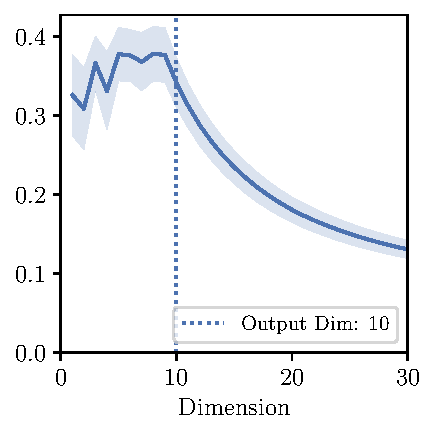
\includegraphics[width=0.23\linewidth]{Appendix_Figures/Overlap_large_model/overlap_raw/last_layer/DimOverlap_MNIST_FC2_fixlr0.01_fc3.pdf}}
%     \subfigure[\centering\small{fc3:LeNet5\\(CIFAR10)}]{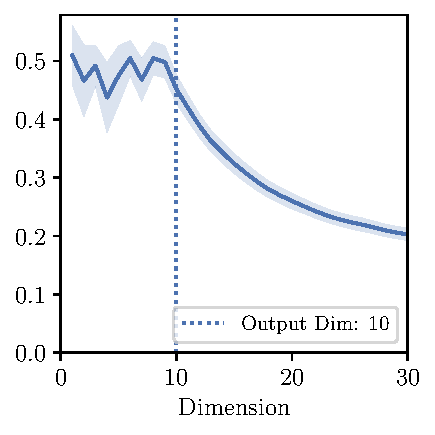
\includegraphics[width=0.23\linewidth]{Appendix_Figures/Overlap_large_model/overlap_raw/last_layer/DimOverlap_CIFAR10_LeNet5_normnew_fixlr0.01_fc3.pdf}}
%     \subfigure[\centering\small{fc1:VGG11-W200\\(CIFAR10)}]{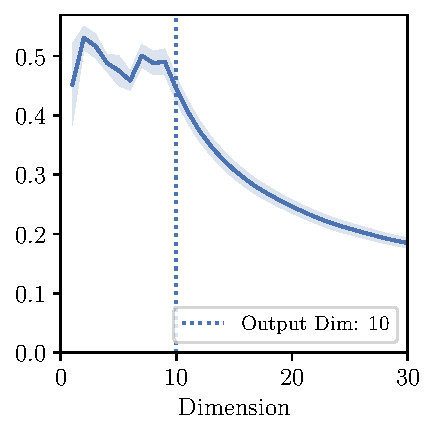
\includegraphics[width=0.23\linewidth]{Appendix_Figures/Overlap_large_model/overlap_raw/last_layer/CIFAR10_VGG11W200_fxlr0.01_fc1.pdf}}
%     \subfigure[\centering\small{fc1:ResNet18-W64\\(CIFAR100)}]{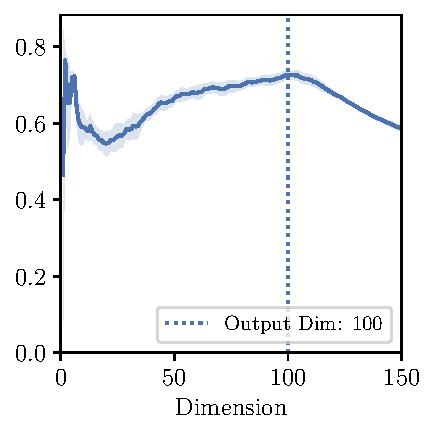
\includegraphics[width=0.23\linewidth]{Appendix_Figures/Overlap_large_model/overlap_raw/last_layer/DimOverlap_CIFAR100_Resnet18W64New_nobn_fixlr0.01_fc1.pdf}}
%     \caption{Top eigenspace overlap for the final fully connected layer.}
%     \label{fig:app_adexp_last}
% \end{figure}

\begin{figure}[H]
    \centering
    \begin{subfigure}[b]{0.24\textwidth}
        \centering
        \captionsetup{justification=centering}
        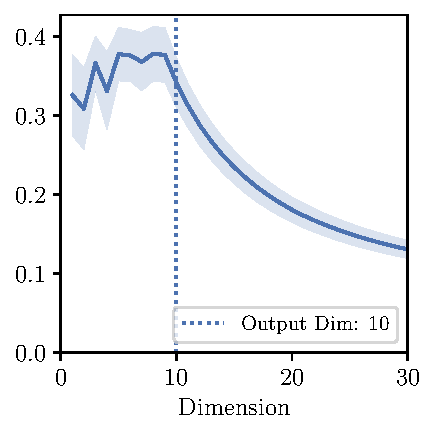
\includegraphics[width=\textwidth]{Appendix_Figures/Overlap_large_model/overlap_raw/last_layer/DimOverlap_MNIST_FC2_fixlr0.01_fc3.pdf}
        \caption{fc3:F-$200^2$\\(MNIST)}
        \label{fig:app_adexp_last_fc2}
    \end{subfigure}
    \begin{subfigure}[b]{0.24\textwidth}
        \centering
        \captionsetup{justification=centering}
        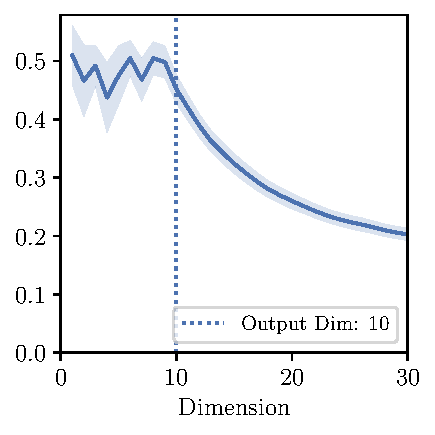
\includegraphics[width=\textwidth]{Appendix_Figures/Overlap_large_model/overlap_raw/last_layer/DimOverlap_CIFAR10_LeNet5_normnew_fixlr0.01_fc3.pdf}
        \caption{fc3:LeNet5\\(CIFAR10)}
        \label{fig:app_adexp_last_LeNet}
    \end{subfigure}
    \begin{subfigure}[b]{0.24\textwidth}
        \centering
        \captionsetup{justification=centering}
        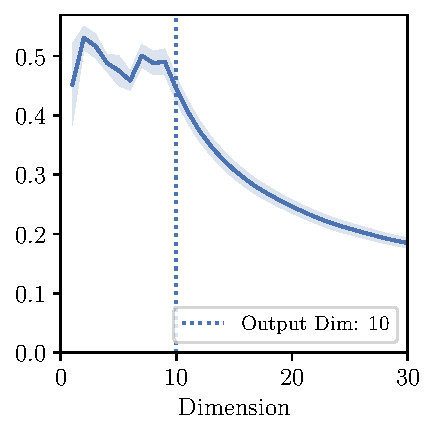
\includegraphics[width=\textwidth]{Appendix_Figures/Overlap_large_model/overlap_raw/last_layer/CIFAR10_VGG11W200_fxlr0.01_fc1.pdf}
        \caption{fc1:VGG11-W200\\(CIFAR10)}
        \label{fig:app_adexp_last_vgg}
    \end{subfigure}
    \begin{subfigure}[b]{0.24\textwidth}
        \centering
        \captionsetup{justification=centering}
        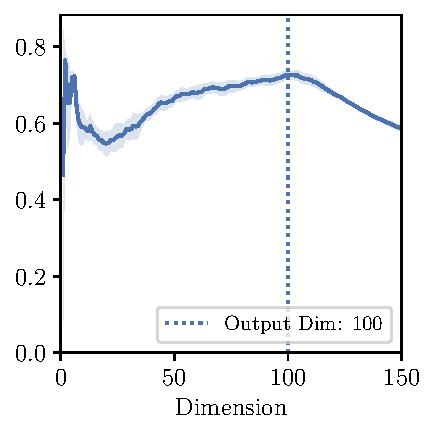
\includegraphics[width=\textwidth]{Appendix_Figures/Overlap_large_model/overlap_raw/last_layer/DimOverlap_CIFAR100_Resnet18W64New_nobn_fixlr0.01_fc1.pdf}
        \caption{fc1:ResNet18-W64\\(CIFAR100)}
        \label{fig:app_adexp_last_resnet}
    \end{subfigure}
    \captionsetup{justification=centering}
    \caption{Top eigenspace overlap for the final fully connected layer.}
    \label{fig:app_adexp_last}
\end{figure}

% \newpage

\subsubsection{Explaining ``Failed Cases'' of Eigenspace Overlap}
\label{sec:appendix-failure}
As shown in \figureref{fig:app_adexp_failure_early} and \figureref{fig:app_adexp_failure_late}, the nontrivial top eigenspace overlap does not necessarily peak at the output dimension for all layers. Some layers has a low peak at very small dimensions and others has a peak at a larger dimension. With the more complete analysis provided above, we now proceed to explain these two phenomenons.
The major reason for such phenomenons is that the assumption of autocorrelation matrix being sufficiently close to rank 1 is not always satisfied. In particular, following the notations in \theoremref{thm:model_overlap}, for these exceptional layers we have $\tau_m\gamma_1 < \tau_1\gamma_2$.
We first consider the first phenomenon (early peak of low overlap) and take fc2:F-$200^2$ (MNIST) in as an example. Here \figureref{fig:app_adexp_fc2}(a) is identical to \figureref{fig:app_adexp_failure_early}(a), which displays the early peak around $m=10$.

% \begin{figure}[H]
%     \centering
%     \subfigure[\centering\small{Eigenspace overlap (zoomed in)}]{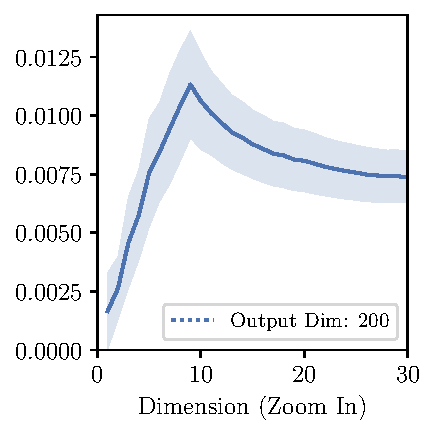
\includegraphics[width=0.24\linewidth]{Appendix_Figures/Overlap_large_model/FailExplanation/FC2/DimOverlap_MNIST_FC2_fixlr0.01_fc2_zoom.pdf}}
%     \subfigure[\centering\small{Eigenspectrum of $\E[\mM]$ and $\E[\vx\vx^\T]$}]{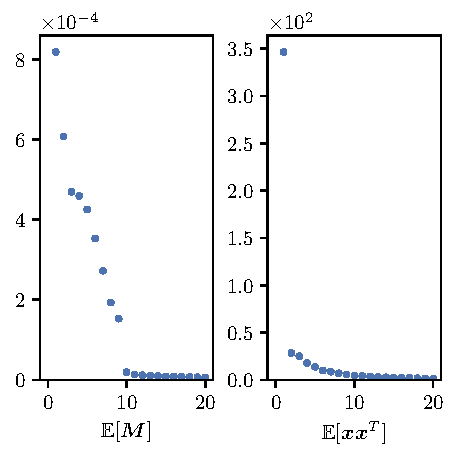
\includegraphics[width=0.24\linewidth]{Appendix_Figures/Overlap_large_model/FailExplanation/FC2/sigvals_t20_MNIST_Exp1_FC2_fixlr0.01R1_E-1_fc2.pdf}}
%     \subfigure[\centering\small{True Hessian with $\E[\vx\vx^\T]$}]{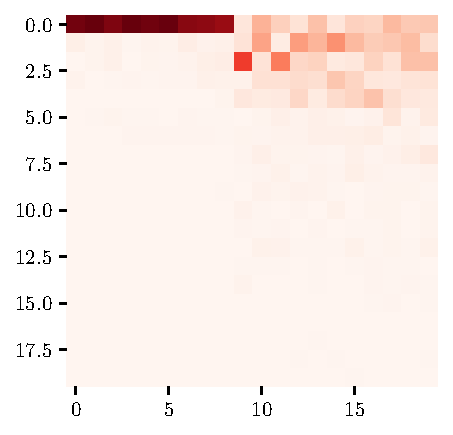
\includegraphics[width=0.24\linewidth]{Appendix_Figures/Overlap_large_model/FailExplanation/FC2/xxT_Trueest_real_corr_expand_t20_MNIST_Exp1_FC2_fixlr0.01R1_E-1_fc2.pdf}}
%     \subfigure[\centering\small{Approx Hessian with $\E[\vx\vx^\T]$}]{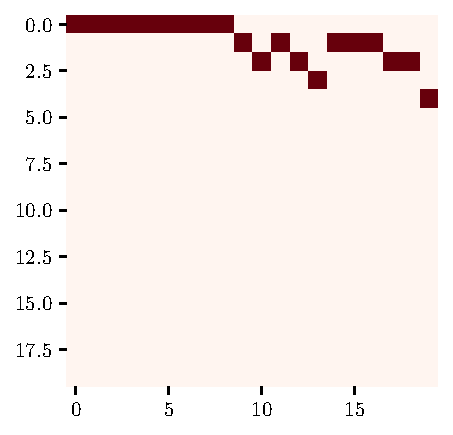
\includegraphics[width=0.24\linewidth]{Appendix_Figures/Overlap_large_model/FailExplanation/FC2/xxT_Approxest_real_corr_expand_t20_MNIST_Exp1_FC2_fixlr0.01R1_E-1_fc2.pdf}}
%     \caption{Eigenspace overlap, eigenspectrum, and cropped (upper $20\times 20$ block)\\eigenvector correspondence matrices for fc2:F-$200^2$ (MNIST)}
%     \label{fig:app_adexp_fc2}
%     \vspace{-2em}
% \end{figure}
% \begin{figure}[H]
%     \centering
%     \subfigure[\centering\small{Eigenspace overlap (zoomed in)}]{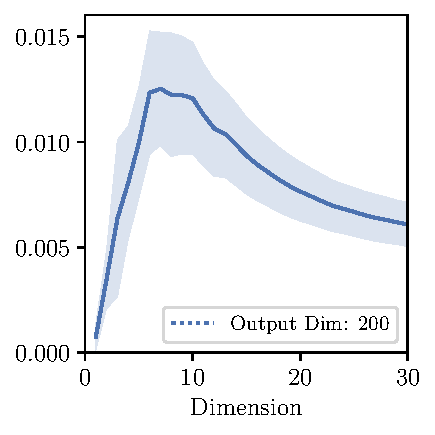
\includegraphics[width=0.24\linewidth]{Appendix_Figures/Overlap_large_model/FailExplanation/VGGearly/DimOverlap_CIFAR10_VGG11W200_fxlr0.01_conv5_zoom.pdf}}
%     \subfigure[\centering\small{Eigenspectrum of $\E[\mM]$ and $\E[\vx\vx^\T]$}]{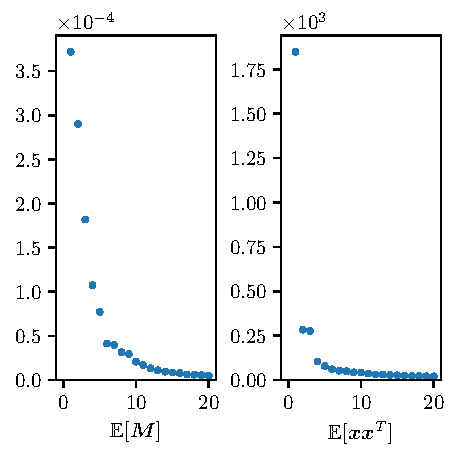
\includegraphics[width=0.24\linewidth]{Appendix_Figures/Overlap_large_model/FailExplanation/VGGearly/sigvals_t20_CIFAR10_Exp1_VGG11W200_fxlr0.01_E-1_features.11.pdf}}
%     \subfigure[\centering\small{True Hessian with $\E[\vx\vx^\T]$}]{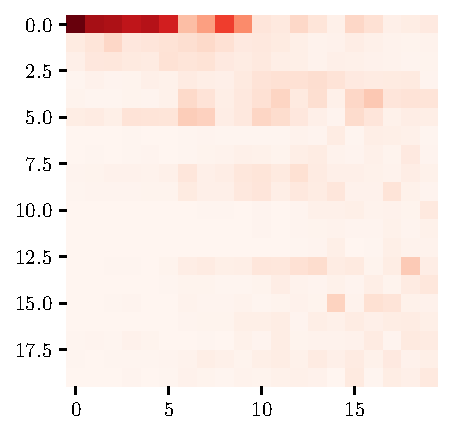
\includegraphics[width=0.24\linewidth]{Appendix_Figures/Overlap_large_model/FailExplanation/VGGearly/xxT_Trueest_real_corr_expand_t20_CIFAR10_Exp1_VGG11W200_fxlr0.01_E-1_features.11.pdf}}
%     \subfigure[\centering\small{Approximated Hessian with $\E[\vx\vx^\T]$}]{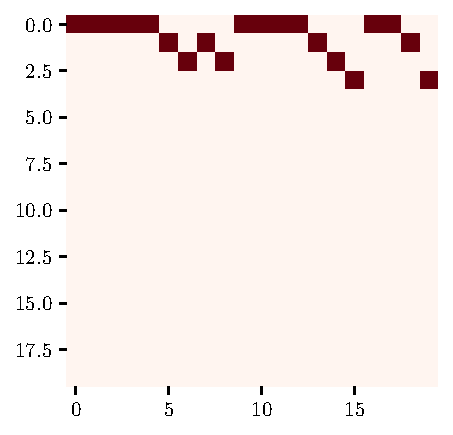
\includegraphics[width=0.24\linewidth]{Appendix_Figures/Overlap_large_model/FailExplanation/VGGearly/xxT_Approxest_real_corr_expand_t20_CIFAR10_Exp1_VGG11W200_fxlr0.01_E-1_features.11.pdf}}
%     \caption{Eigenspace overlap, eigenspectrum, and cropped (upper $20\times 20$ block)\\eigenvector correspondence matrices for conv5:VGG11-W200 (CIFAR10)}
%     \vspace{-0.1in}
%     \label{fig:app_adexp_vgg_fail}
% \end{figure}
\begin{figure}[H]
    \centering
    \begin{subfigure}[b]{0.24\textwidth}
        \centering
        \captionsetup{justification=centering}
        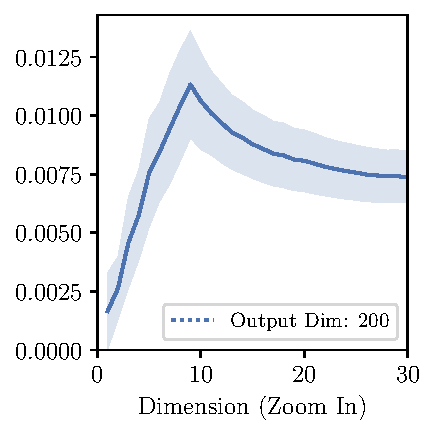
\includegraphics[width=\textwidth]{Appendix_Figures/Overlap_large_model/FailExplanation/FC2/DimOverlap_MNIST_FC2_fixlr0.01_fc2_zoom.pdf}
        \caption{Eigenspace overlap (zoomed in)}
        \label{fig:app_adexp_fc2_ovlp}
    \end{subfigure}%
    \begin{subfigure}[b]{0.24\textwidth}
        \centering
        \captionsetup{justification=centering}
        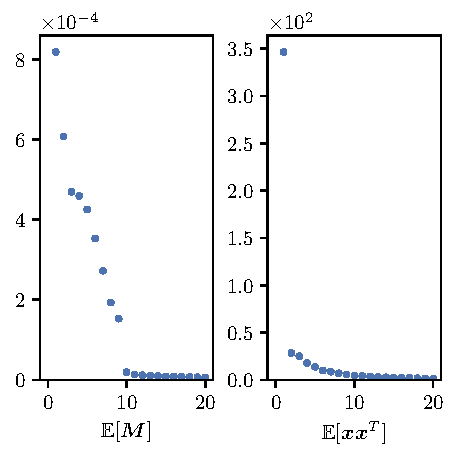
\includegraphics[width=\textwidth]{Appendix_Figures/Overlap_large_model/FailExplanation/FC2/sigvals_t20_MNIST_Exp1_FC2_fixlr0.01R1_E-1_fc2.pdf}
        \caption{Eigenspectrum of $\E[\mM]$ and $\E[\vx\vx^\T]$}
        \label{fig:app_adexp_fc2_sig}
    \end{subfigure}%
    \begin{subfigure}[b]{0.24\textwidth}
        \centering
        \captionsetup{justification=centering}
        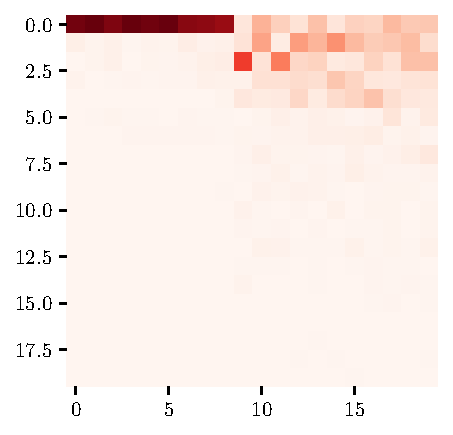
\includegraphics[width=\textwidth]{Appendix_Figures/Overlap_large_model/FailExplanation/FC2/xxT_Trueest_real_corr_expand_t20_MNIST_Exp1_FC2_fixlr0.01R1_E-1_fc2.pdf}
        \caption{True Hessian with $\E[\vx\vx^\T]$}
        \label{fig:app_adexp_fc2_corr_real}
    \end{subfigure}
    \begin{subfigure}[b]{0.24\textwidth}
        \centering
        \captionsetup{justification=centering}
        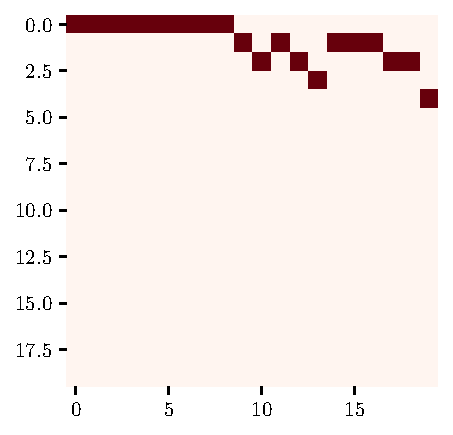
\includegraphics[width=\textwidth]{Appendix_Figures/Overlap_large_model/FailExplanation/FC2/xxT_Approxest_real_corr_expand_t20_MNIST_Exp1_FC2_fixlr0.01R1_E-1_fc2.pdf}
        \caption{Approximated Hessian with $\E[\vx\vx^\T]$}
        \label{fig:app_adexp_fc2_corr_est}
    \end{subfigure}
    \captionsetup{justification=centering}
    \caption{Eigenspace overlap, eigenspectrum, and cropped (upper $20\times 20$ block)\\eigenvector correspondence matrices for fc2:F-$200^2$ (MNIST)}
    \vspace{-0.1in}
    \label{fig:app_adexp_fc2}
\end{figure}

\begin{figure}[H]
    \centering
    \begin{subfigure}[b]{0.24\textwidth}
        \centering
        \captionsetup{justification=centering}
        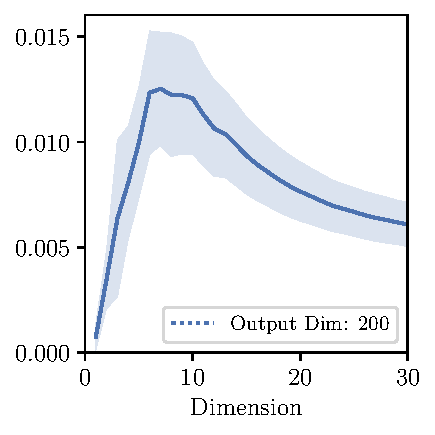
\includegraphics[width=\textwidth]{Appendix_Figures/Overlap_large_model/FailExplanation/VGGearly/DimOverlap_CIFAR10_VGG11W200_fxlr0.01_conv5_zoom.pdf}
        \caption{Eigenspace overlap (zoomed in)}
        \label{fig:app_adexp_vgg_ovlp}
    \end{subfigure}%
    \begin{subfigure}[b]{0.24\textwidth}
        \centering
        \captionsetup{justification=centering}
        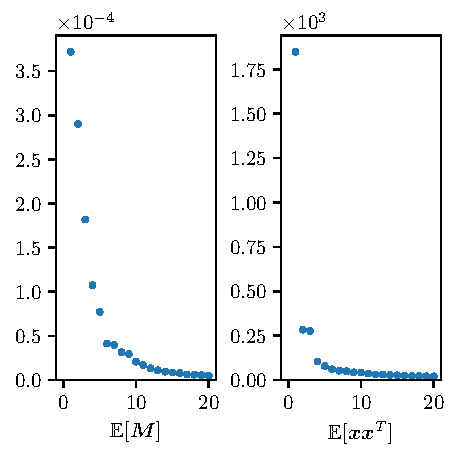
\includegraphics[width=\textwidth]{Appendix_Figures/Overlap_large_model/FailExplanation/VGGearly/sigvals_t20_CIFAR10_Exp1_VGG11W200_fxlr0.01_E-1_features.11.pdf}
        \caption{Eigenspectrum of $\E[\mM]$ and $\E[\vx\vx^\T]$}
        \label{fig:app_adexp_vgg_sig}
    \end{subfigure}%
    \begin{subfigure}[b]{0.24\textwidth}
        \centering
        \captionsetup{justification=centering}
        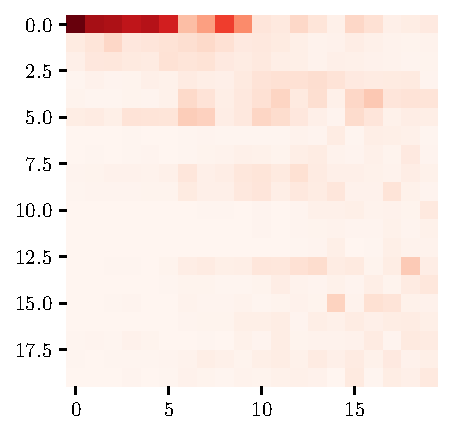
\includegraphics[width=\textwidth]{Appendix_Figures/Overlap_large_model/FailExplanation/VGGearly/xxT_Trueest_real_corr_expand_t20_CIFAR10_Exp1_VGG11W200_fxlr0.01_E-1_features.11.pdf}
        \caption{True Hessian with $\E[\vx\vx^\T]$}
        \label{fig:app_adexp_vgg_corr_real}
    \end{subfigure}
    \begin{subfigure}[b]{0.24\textwidth}
        \centering
        \captionsetup{justification=centering}
        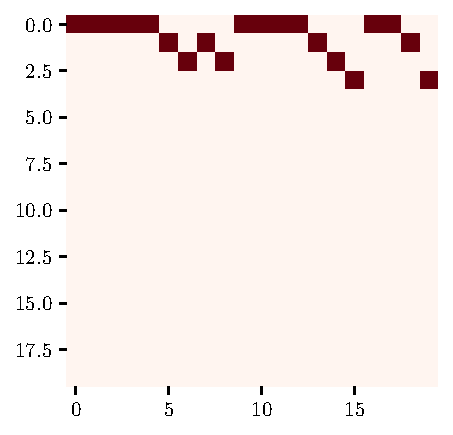
\includegraphics[width=\textwidth]{Appendix_Figures/Overlap_large_model/FailExplanation/VGGearly/xxT_Approxest_real_corr_expand_t20_CIFAR10_Exp1_VGG11W200_fxlr0.01_E-1_features.11.pdf}
        \caption{Approximated Hessian with $\E[\vx\vx^\T]$}
        \label{fig:app_adexp_vgg_corr_est}
    \end{subfigure}
    \captionsetup{justification=centering}
    \caption{Eigenspace overlap, eigenspectrum, and cropped (upper $50\times 50$ block)\\eigenvector correspondence matrices for conv2:VGG11-W200 (CIFAR10)}
    \vspace{-0.1in}
    \label{fig:app_adexp_vgg_fail}
\end{figure}

As shown in \figureref{fig:app_adexp_fc2}(b), the second eigenvalue of the auto correlation $\E[\vx\vx^\T]$ is as large as approximately 1/10 of the first eigenvalue.
With the output Hessian have $c-1=9$ significant large eigenvalues as described in \label{sec:emp_outlier}, it has $\tau_{10}\gamma_1 < \tau_1\gamma_2$.
Thus through the Kronecker factorization approximation, the top $m$ dimensional eigenspace is no longer simply $\mI_m\otimes \hE[\vx]$, but a subset of top eigenvectors of the output Hessian Kroneckered with a subset of top eigenvectors of $\E[\vx\vx^\T]$ as reflected in \figureref{fig:app_adexp_fc2}(d). This ``mixture'' of Kronecker product is moreover verified in \figureref{fig:app_adexp_fc2}(c).

As reflected by the first row of \figureref{fig:app_adexp_fc2}(c) and \figureref{fig:app_adexp_fc2}(d), for $i\leq 9$ we have $\vh_i\approx \vr_i\otimes\hE[\vx]$, which falls in the regime of \theoremref{thm:model_overlap}. Hence we are seeing an linearly growing pattern of the overlap for dimension less than 10 and reaches a mean overlap of around 0.012 by dimension 9. If following this linear trend, the overlap would be close to 0.25 by the output dimension of 200. However, since the 10-th eigenvalue of the output Hessian is significantly smaller, little of the 10-19 dimensional eigenspace were contributed by $\hE[\vx]$, hence the overlap of dimension larger than 10 falls into the regime discussed in \sectionref{sec:app_ovlp_dec}, for which we see a sharp decrease of overlap after dimension 9.
Note that this example shows that Kronecker factorization can be used to predict when our conditions in \theoremref{thm:model_overlap} fails and also predict the condition can be satisfied up to which dimension. As shown in \figureref{fig:app_adexp_vgg_fail}, similar explanation also applies to convolutional layers in larger networks.



% \begin{figure}[H]
%     \centering
%     \begin{subfigure}[b]{0.24\textwidth}
%         \centering
%         \captionsetup{justification=centering}
%         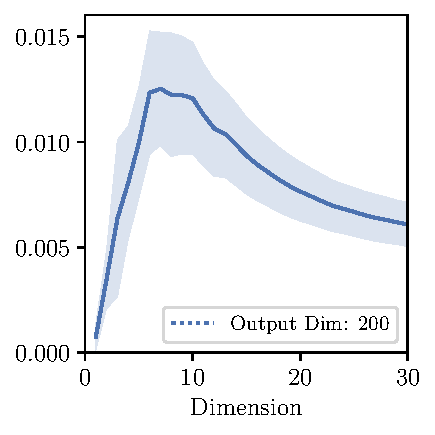
\includegraphics[width=\textwidth]{Appendix_Figures/Overlap_large_model/FailExplanation/VGGearly/DimOverlap_CIFAR10_VGG11W200_fxlr0.01_conv5_zoom.pdf}
%         \caption{Eigenspace overlap (zoomed in)}
%         \label{fig:app_adexp_vgg_ovlp}
%     \end{subfigure}%
%     \begin{subfigure}[b]{0.24\textwidth}
%         \centering
%         \captionsetup{justification=centering}
%         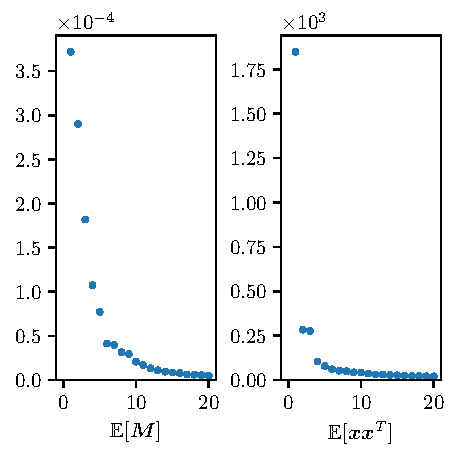
\includegraphics[width=\textwidth]{Appendix_Figures/Overlap_large_model/FailExplanation/VGGearly/sigvals_t20_CIFAR10_Exp1_VGG11W200_fxlr0.01_E-1_features.11.pdf}
%         \caption{Eigenspectrum of $\E[\mM]$ and $\E[\vx\vx^\T]$}
%         \label{fig:app_adexp_vgg_sig}
%     \end{subfigure}%
%     \begin{subfigure}[b]{0.24\textwidth}
%         \centering
%         \captionsetup{justification=centering}
%         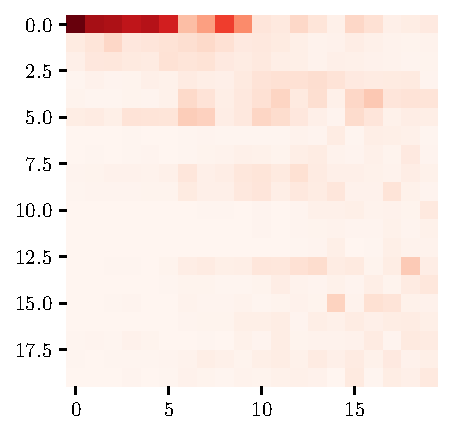
\includegraphics[width=\textwidth]{Appendix_Figures/Overlap_large_model/FailExplanation/VGGearly/xxT_Trueest_real_corr_expand_t20_CIFAR10_Exp1_VGG11W200_fxlr0.01_E-1_features.11.pdf}
%         \caption{True Hessian with $\E[\vx\vx^\T]$}
%         \label{fig:app_adexp_vgg_corr_real}
%     \end{subfigure}
%     \begin{subfigure}[b]{0.24\textwidth}
%         \centering
%         \captionsetup{justification=centering}
%         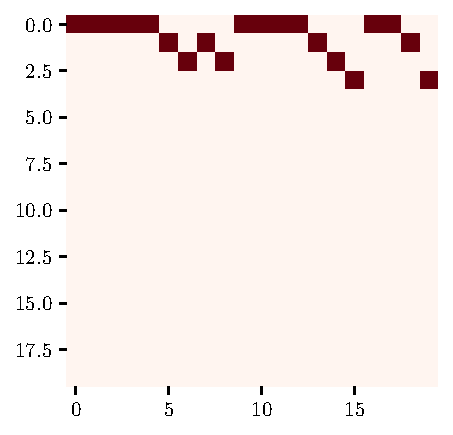
\includegraphics[width=\textwidth]{Appendix_Figures/Overlap_large_model/FailExplanation/VGGearly/xxT_Approxest_real_corr_expand_t20_CIFAR10_Exp1_VGG11W200_fxlr0.01_E-1_features.11.pdf}
%         \caption{Approximated Hessian with $\E[\vx\vx^\T]$}
%         \label{fig:app_adexp_vgg_corr_est}
%     \end{subfigure}
%     \captionsetup{justification=centering}
%     \caption{Eigenspace overlap, eigenspectrum, and cropped (upper $20\times 20$ block)\\eigenvector correspondence matrices for conv5:VGG11-W200 (CIFAR10)}
%     \vspace{-0.1in}
%     \label{fig:app_adexp_vgg}
% \end{figure}

We then consider the second phenomenon (delayed peak) and take conv2:VGG11-W200 (CIFAR10) in as an example. Here \figureref{fig:app_adexp_vgg2}(a) is identical to \figureref{fig:app_adexp_failure_late}(d), which has the overlap peak later than the output dimension 200. In this case, the second eigenvalue of the auto correlation matrix is still not negligible compared to the top eigenvalue. What differentiate this case from the first phenomenon is that the eigenvalues of the output Hessian no longer has a significant peak \--- instead it has a heavy tail which is necessary for high overlap.

Towards dimension $m$ there gradually exhibits higher correspondence to later eigenvectors of the input autocorrelation matrix and hence less correspondence to $\hE[\vx]$. This eventually results in the delayed and flattened peak.


% \begin{figure}[H]
%     \centering
%     \subfigure[\centering\small{Eigenspace overlap\\ (zoomed in)}]{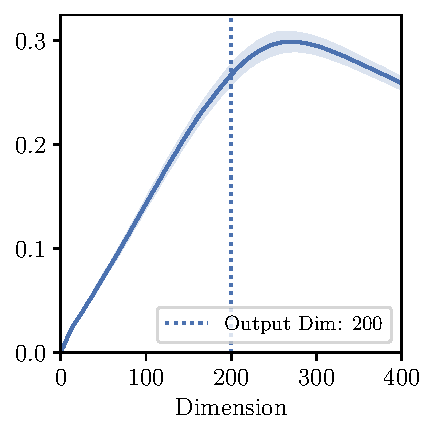
\includegraphics[width=0.23\linewidth]{Appendix_Figures/Overlap_large_model/FailCases/late/CIFAR10_VGG11W200_fxlr0.01_conv2.pdf}}
%     \subfigure[\centering\small{Eigenspectrum of\\ $\E[\mM]$ and $\E[\vx\vx^\T]$}]{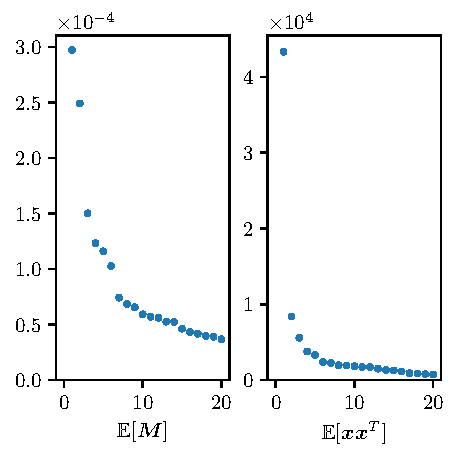
\includegraphics[width=0.23\linewidth]{Appendix_Figures/Overlap_large_model/FailExplanation/VGGlate/sigvals_t20_CIFAR10_Exp1_VGG11W200_fxlr0.01_E-1_features.3.pdf}}
%     \subfigure[\centering\small{True Hessian\\ with $\E[\vx\vx^\T]$}]{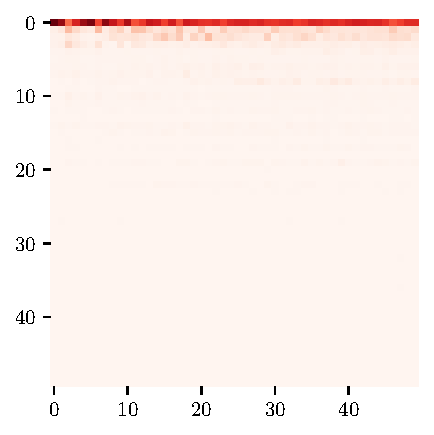
\includegraphics[width=0.23\linewidth]{Appendix_Figures/Overlap_large_model/FailExplanation/VGGlate/xxT_Trueest_real_corr_expand_t50_CIFAR10_Exp1_VGG11W200_fxlr0.01_E-1_features.3.pdf}}
%     \subfigure[\centering\small{Approx Hessian\\ with $\E[\vx\vx^\T]$}]{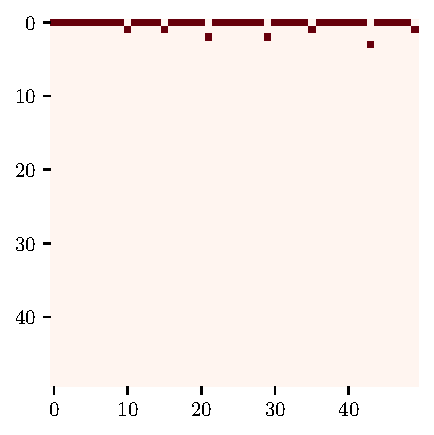
\includegraphics[width=0.23\linewidth]{Appendix_Figures/Overlap_large_model/FailExplanation/VGGlate/xxT_Approxest_real_corr_expand_t50_CIFAR10_Exp1_VGG11W200_fxlr0.01_E-1_features.3.pdf}}\\
%     \vspace{0.15in}
%     \subfigure[\centering\small{First Row of Correspondence Matrix\\ of True Hessian with $\E[\vx\vx^\T]$}]{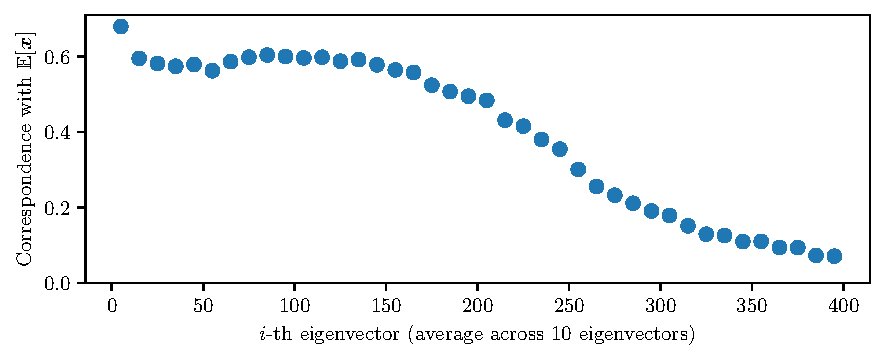
\includegraphics[width=0.49\linewidth]{Appendix_Figures/Overlap_large_model/FailExplanation/VGGlate/FL_xxT_Trueest_real_corr_expand_t400_CIFAR10_Exp1_VGG11W200_fxlr0.01_E-1_features.3.pdf}}
%     \subfigure[\centering\small{First Row of Correspondence Matrix of\\ Approximated Hessian with $\E[\vx\vx^\T]$}]{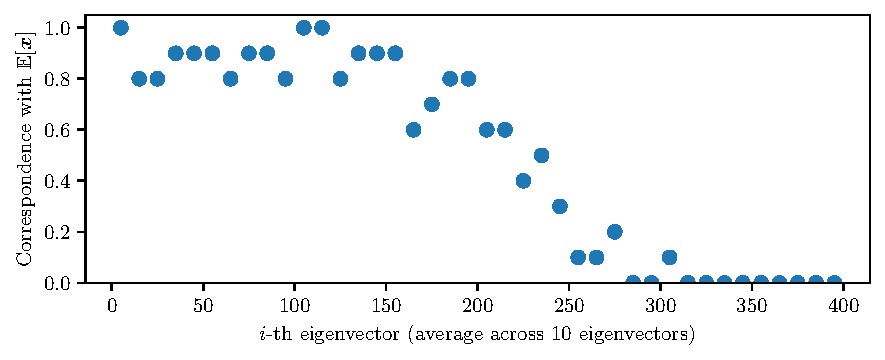
\includegraphics[width=0.49\linewidth]{Appendix_Figures/Overlap_large_model/FailExplanation/VGGlate/FL_xxT_Approxest_real_corr_expand_t400_CIFAR10_Exp1_VGG11W200_fxlr0.01_E-1_features.3.pdf}}
%     \caption{Eigenspace overlap, eigenspectrum, and cropped (upper $50\times 50$ block)\\eigenvector correspondence matrices for conv2:VGG11-W200 (CIFAR10)}
%     \label{fig:app_adexp_vgg2}
%     % \vspace{-1em}
% \end{figure}

\begin{figure}[H]
    \centering
    \begin{subfigure}[b]{0.24\textwidth}
        \centering
        \captionsetup{justification=centering}
        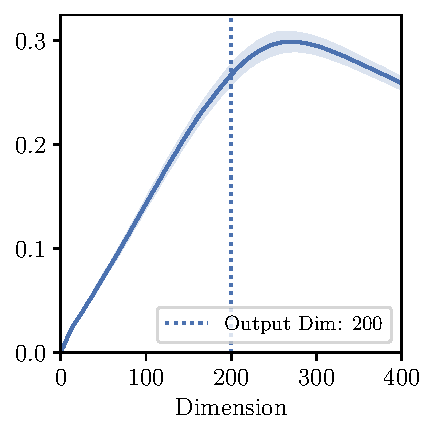
\includegraphics[width=\textwidth]{Appendix_Figures/Overlap_large_model/FailCases/late/CIFAR10_VGG11W200_fxlr0.01_conv2.pdf}
        \caption{Eigenspace overlap (zoomed in)}
        \label{fig:app_adexp_vgg2_ovlp}
    \end{subfigure}%
    \begin{subfigure}[b]{0.24\textwidth}
        \centering
        \captionsetup{justification=centering}
        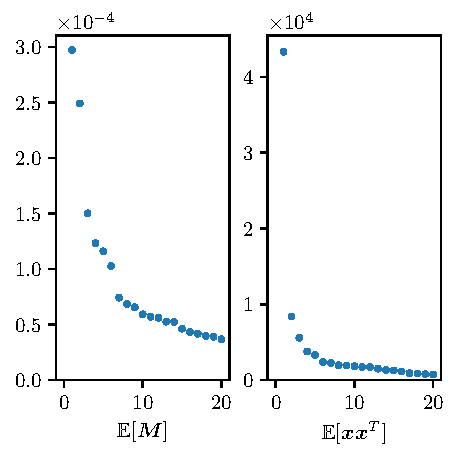
\includegraphics[width=\textwidth]{Appendix_Figures/Overlap_large_model/FailExplanation/VGGlate/sigvals_t20_CIFAR10_Exp1_VGG11W200_fxlr0.01_E-1_features.3.pdf}
        \caption{Eigenspectrum of $\E[\mM]$ and $\E[\vx\vx^\T]$}
        \label{fig:app_adexp_vgg2_sig}
    \end{subfigure}%
    \begin{subfigure}[b]{0.24\textwidth}
        \centering
        \captionsetup{justification=centering}
        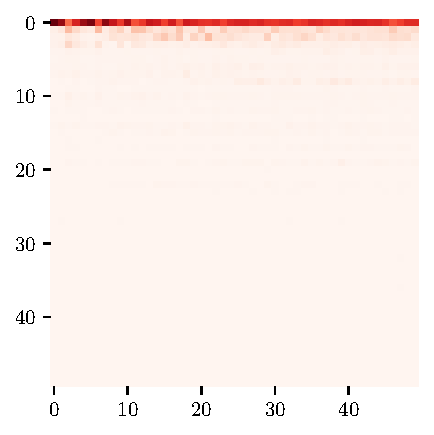
\includegraphics[width=\textwidth]{Appendix_Figures/Overlap_large_model/FailExplanation/VGGlate/xxT_Trueest_real_corr_expand_t50_CIFAR10_Exp1_VGG11W200_fxlr0.01_E-1_features.3.pdf}
        \caption{True Hessian with $\E[\vx\vx^\T]$}
        \label{fig:app_adexp_vgg2_corr_real}
    \end{subfigure}
    \begin{subfigure}[b]{0.24\textwidth}
        \centering
        \captionsetup{justification=centering}
        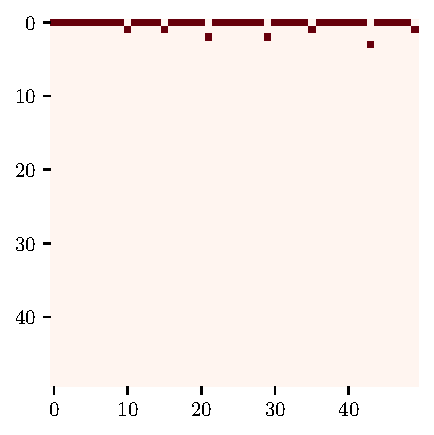
\includegraphics[width=\textwidth]{Appendix_Figures/Overlap_large_model/FailExplanation/VGGlate/xxT_Approxest_real_corr_expand_t50_CIFAR10_Exp1_VGG11W200_fxlr0.01_E-1_features.3.pdf}
        \caption{Approximated Hessian with $\E[\vx\vx^\T]$}
        \label{fig:app_adexp_vgg2_corr_est}
    \end{subfigure}\\
    \vspace{0.15in}
    \begin{subfigure}[b]{0.49\textwidth}
        \centering
        \captionsetup{justification=centering}
        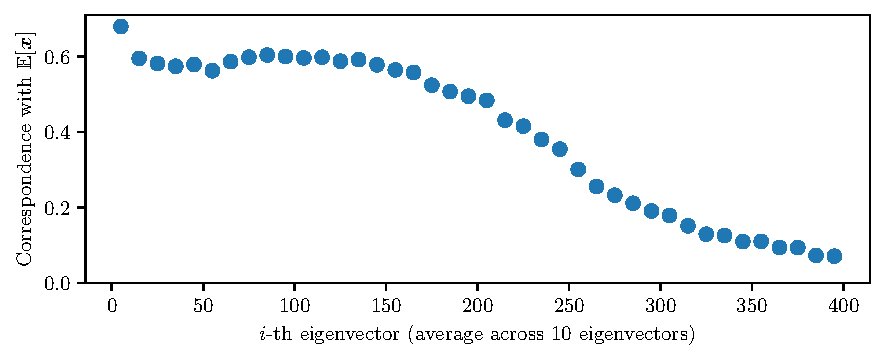
\includegraphics[width=\textwidth]{Appendix_Figures/Overlap_large_model/FailExplanation/VGGlate/FL_xxT_Trueest_real_corr_expand_t400_CIFAR10_Exp1_VGG11W200_fxlr0.01_E-1_features.3.pdf}
        \caption{First Row of Correspondence Matrix of True Hessian with $\E[\vx\vx^\T]$}
        \label{fig:app_adexp_vgg2_corr_true_firstline}
    \end{subfigure}
    \begin{subfigure}[b]{0.49\textwidth}
        \centering
        \captionsetup{justification=centering}
        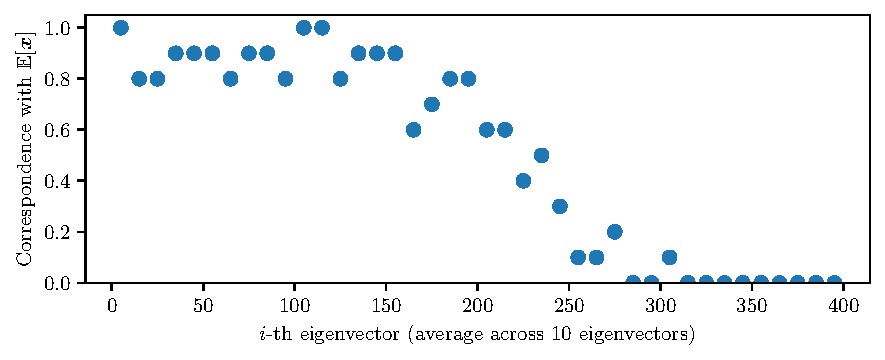
\includegraphics[width=\textwidth]{Appendix_Figures/Overlap_large_model/FailExplanation/VGGlate/FL_xxT_Approxest_real_corr_expand_t400_CIFAR10_Exp1_VGG11W200_fxlr0.01_E-1_features.3.pdf}
        \caption{First Row of Correspondence Matrix of Approximated Hessian with $\E[\vx\vx^\T]$}
        \label{fig:app_adexp_vgg2_corr_est_firstline}
    \end{subfigure}
    \captionsetup{justification=centering}
    \caption{Eigenspace overlap, eigenspectrum, and cropped (upper $50\times 50$ block)\\eigenvector correspondence matrices for conv2:VGG11-W200 (CIFAR10)}
    \vspace{-0.1in}
    \label{fig:app_adexp_vgg2}
\end{figure}

Since the full correspondence matrices are too large to be visualized, we plotted their first rows up to 400 dimensions in \figureref{fig:app_adexp_vgg2}(e) and \figureref{fig:app_adexp_vgg2}(f), in which each dot represents the average of correlation with $\hE[\vx]$ for the 10 eigenvector nearby. From these figures it is straightforward to see the gradual decreasing correlation with $\hE[\vx].$
% We can explain this case by looking at the eigenvector correspondence matrices shown in \figureref{fig:app_adexp_fc2}. The correspondence between eigenvectors of layer-wise Hessian and the top eigenvector of $\E[\vx\vx^\T]$ is only close to 1 for the top 9 eigenvectors. Thus, \theoremref{thm:model_overlap} does not apply here. However, we can observe a small peak at dimension 9 and linear growth before it, as shown in \figureref{fig:app_adexp_fc2_ovlp}. This is because our approximation can still be applied before dimension 9. Demonstrating that eigenspace overlap of different models can be predicted using eigenvector correspondence matrices.

% \begin{figure}[ht]
%     \centering
%     \begin{subfigure}[b]{0.24\textwidth}
%         \centering
%         \captionsetup{justification=centering}
%         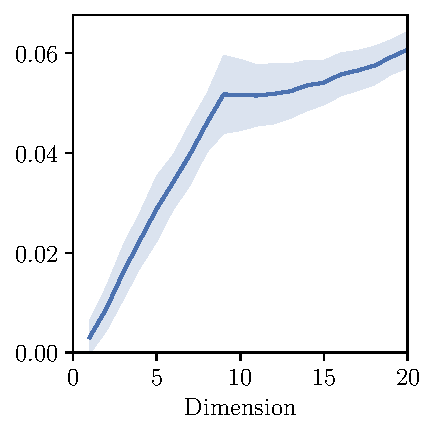
\includegraphics[width=\textwidth]{Appendix_Figures/Explanation_LeNet5Case/fc2_corr/DimOverlap_CIFAR10_LeNet5_normnew_fixlr0.01_fc2_xlim20.pdf}
%         \caption{Eigenspace overlap (zoomed in)}
%         \label{fig:app_adexp_fc2_ovlp}
%     \end{subfigure}%
%     \begin{subfigure}[b]{0.24\textwidth}
%         \centering
%         \captionsetup{justification=centering}
%         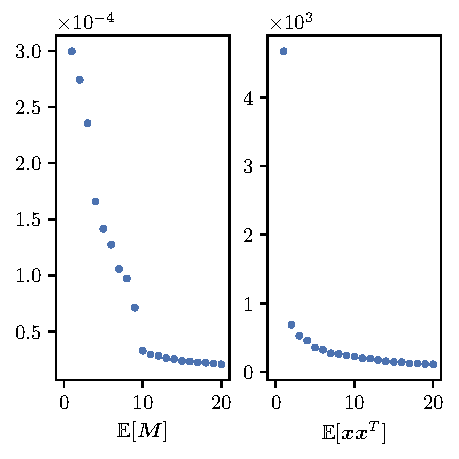
\includegraphics[width=\textwidth]{Appendix_Figures/Explanation_LeNet5Case/fc2_corr/sigvals_t20_CIFAR10_Exp1_LeNet5_normnew_fixlr0.01R2_E-1_fc2.pdf}
%         \caption{Eigenspectrum of $\E[\mM]$ and $\E[\vx\vx^\T]$}
%         \label{fig:app_adexp_fc2_sig}
%     \end{subfigure}%
%     \begin{subfigure}[b]{0.24\textwidth}
%         \centering
%         \captionsetup{justification=centering}
%         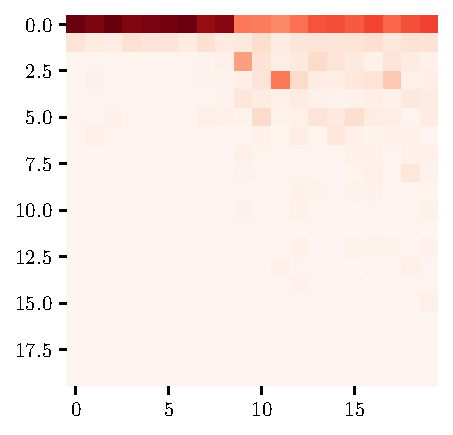
\includegraphics[width=\textwidth]{Appendix_Figures/Explanation_LeNet5Case/fc2_corr/xxT_Trueest_real_corr_expand_t20_CIFAR10_Exp1_LeNet5_normnew_fixlr0.01R2_E-1_fc2.pdf}
%         \caption{True Hessian with $E[\vx\vx^\T]$}
%         \label{fig:app_adexp_fc2_corr_real}
%     \end{subfigure}
%     \begin{subfigure}[b]{0.24\textwidth}
%         \centering
%         \captionsetup{justification=centering}
%         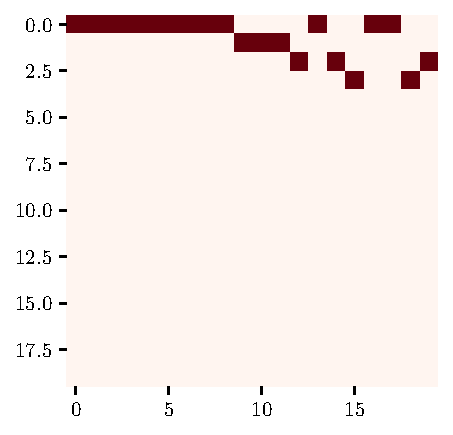
\includegraphics[width=\textwidth]{Appendix_Figures/Explanation_LeNet5Case/fc2_corr/xxT_Approxest_real_corr_expand_t20_CIFAR10_Exp1_LeNet5_normnew_fixlr0.01R2_E-1_fc2.pdf}
%         \caption{Approximated Hessian with $E[\vx\vx^\T]$}
%         \label{fig:app_adexp_fc2_corr_est}
%     \end{subfigure}
%     \captionsetup{justification=centering}
%     \caption{Eigenspace overlap, Eigenspectrum, and Eigenvector correspondence matrices for fc2:LeNet5}
%     \label{fig:app_adexp_fc2}
% \end{figure}

% In addition, \figureref{fig:app_adexp_fc2_corr_est} shows the correspondence matrix for the approximated Hessian using Kronekecker factorization $\E[\mM]\otimes \E[\vx\vx^\T]$. Let $\vu_i$ be that of $\E[\mM]$ with corresponding eigenvalue $\lambda_i$. Let $\vv_i$ be the $i$th eigenvector of $\E[\vx\vx^\T]$ with corresponding eigenvalue $\mu_i$. This approximation shows that the top 9 eigenvectors can be approximated as $\vu_i\otimes \vv_1$ for some $\vu_i$ but the 10th eigenvector cannot. Since the eigenvectors are ranked according to the magnitude of their corresponding eigenvalues, which are approximated using products of eigenvalues of $\E[\mM]$ and $\E[\vx\vx^\T]$. This is equivalent to having $\lambda_{10}\mu_1 < \lambda_1\mu_2$. From \figureref{fig:app_adexp_fc2_sig}, we can see that there is a significant gap between $\lambda_9$ and $\lambda_{10}$, suggesting why we have this inequality.



% \paragraph{The cases of large networks: Large second eigenvalue of the input auto-correlation matrix reduces the overlap}

% There is another case when the overlap is not as high as expected. This situation happens in large networks in our experiments. It is when the input auto-correlation matrix $\E[\vx\vx^\T]$ has a large second eigenvalue.

% \begin{figure}[ht]
%     \centering
%     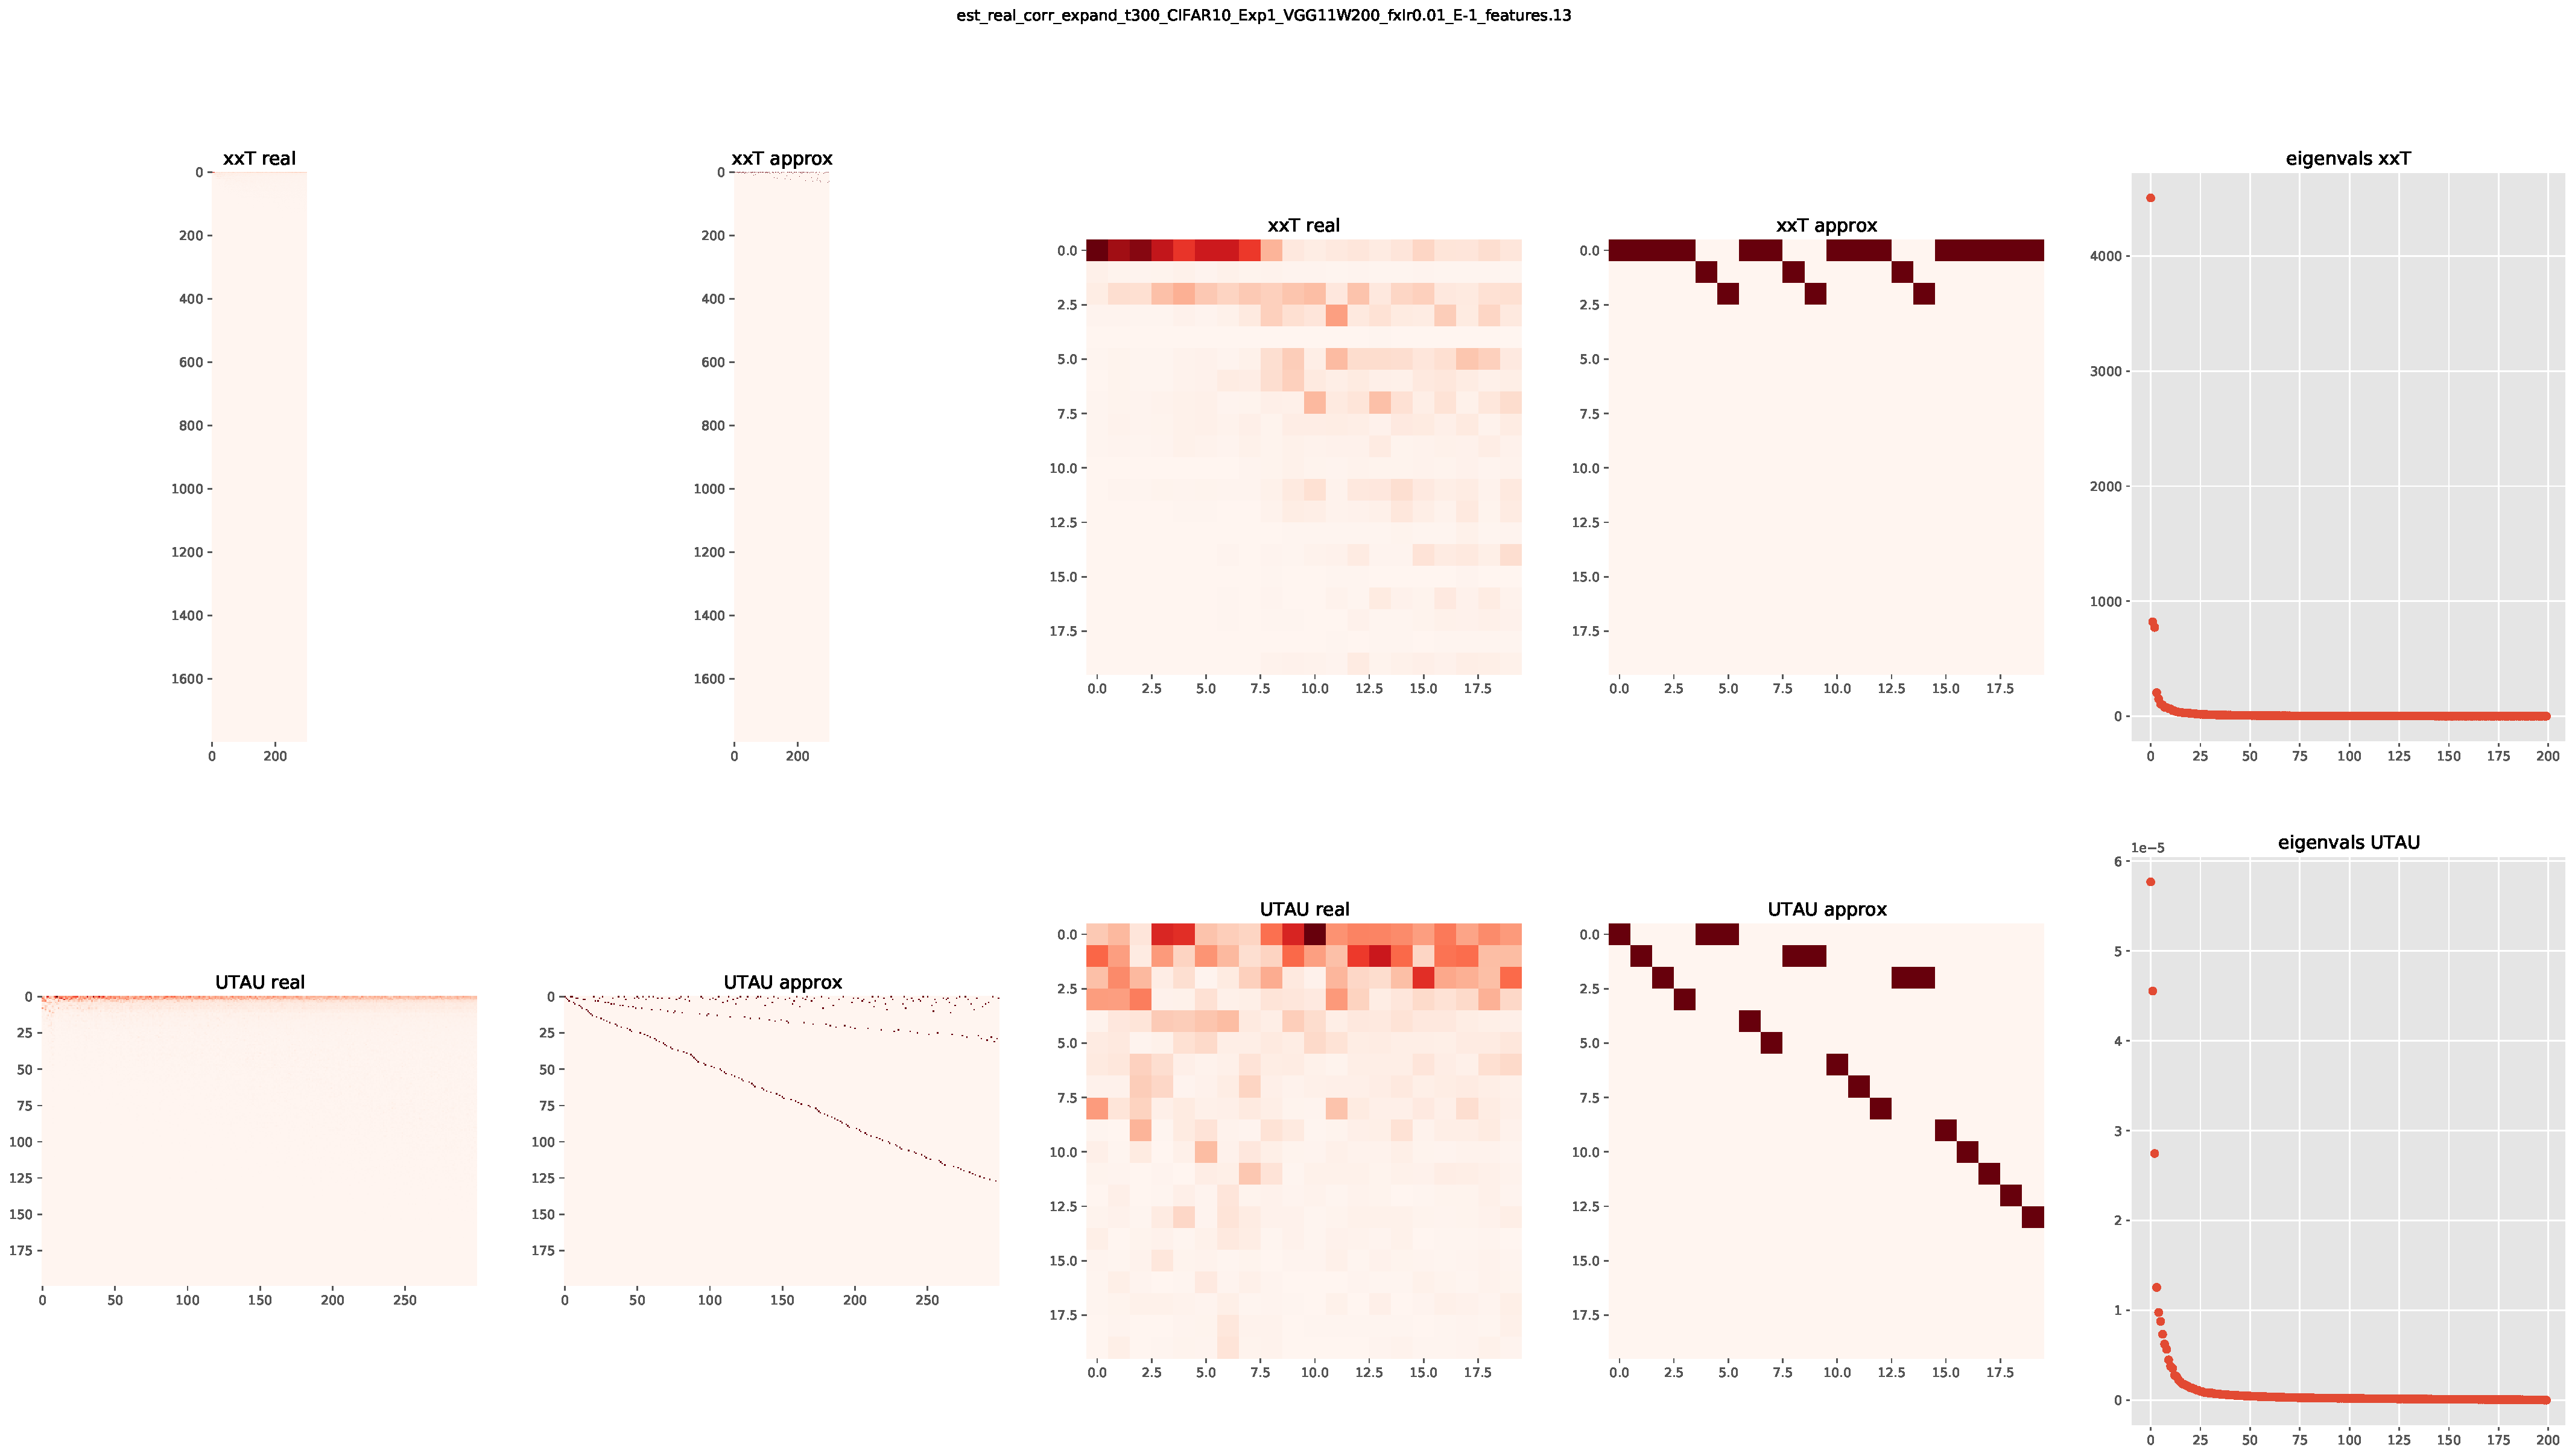
\includegraphics[width=\textwidth]{Appendix_Figures/Overlap_large_model/est_real_corr_expand_t300_CIFAR10_Exp1_VGG11W200_fxlr0.01_E-1_features.13.pdf}
%     \caption{Eigenvector correspondence and eigenspectrum for features.13:VGG11W200}
%     \label{fig:eigenvector_VGG_13}
% \end{figure}

% As we can see in \figureref{fig:eigenvector_VGG_13}, although the eigenspectrum of $\E[\vx\vx^\T]$ has a dominating first eigenvalue, it also have significantly large second and third eigenvalue. As we did in the case above (low rank output Hessian), we let $\vu_i$ be that of $\E[\mM]$ with corresponding eigenvalue $\lambda_i$. Let $\vv_i$ be the $i$th eigenvector of $\E[\vx\vx^\T]$ with corresponding eigenvalue $\mu_i$. In this case, we can see that the top 4 eigenvectors can be approximated as $\vu_i \otimes \vv_1$, but the 5th eigenvector cannot. We have $\lambda_5\mu_1 < \lambda_1\mu_2$. Thus, similar to the case for low rank output Hessian, our condition in \theoremref{thm:model_overlap} fails, which gives the reason why the overlap is not high for this layer. Kronecker factorization and eigenvector correspondence can be used to predict when our condition in \theoremref{thm:model_overlap} fails in both cases. 
